%Results (1p)
\section{Evaluation}
\label{sec:evaluation}

In this section we focus on the evaluation of the proposed approach.
To do so we used the Goal-Question-Metric (GQM) evaluation methodology~\cite{basili_goal_1994}.

As the first step in GQM methodology we defined the following high-level evaluation goal:

Our first evaluation goal G1 is to assess the feasibility of the approach. To do so, we need to evaluate if a software architect/developer can follow the proposed patterns to refine a goal-model into components and artifacts. Also we need to evaluate if the proposed planning algorithm is capable of autonomously creating a reliable deployment plan.
Such an evaluation required the definition of the following questions and metrics:

\begin{itemize}
  \item Q1.1: For the Filling Station Advisor case study, are the goal-component-artifact patterns a feasible approach to map artifacts from the CGM of the case study?
  \begin{itemize}
    \item Map artifacts for the Filling Station Advisor case study using proposed patterns.
  \end{itemize}

  \item Q1.2: How long would the algorithm take to come up with a deployment plan?
  \begin{itemize}
    \item Time to produce a plan.
  \end{itemize}

  \item Q1.3: How reliable would a plan provided
  by the algorithm be?
  \begin{itemize}
    \item Percentage of correct answers.
  \end{itemize}

\end{itemize}

Since the Filling Station Advisor has a limited size and does not allow for controlled factors experiments, our second goal G2 aims to provide a more comprehensible scalability evaluation of Goalp. So we defined the following questions and metrics:

\begin{itemize}
  \item Q2.1: How does the algorithm scale over the number of artifacts in the deployment plan?
  \begin{itemize}
    \item M2.1: The time consumed to come up with a deployment plan.
  \end{itemize}

  \item Q2.2: How does the algorithm scale over the variability level on the repository?
  \begin{itemize}
    \item M2.2: The time consumed to come up with a deployment plan.
  \end{itemize}
\end{itemize}

The experiments were conducted using a laptop computer with Intel i5-3337U, 12GB DDR3 1600MHz memory, and Linux (Kernel 3.16.0-77generic). OracleJDK(1.8.0 91-b14) was used to build and run the project. All experiments were implemented in Java and are available.
\footnote{The evaluation experiments and the complete result set are available at
\url{https://github.com/lesunb/goalp} Accessed on November 5th, 2016}
All experiments to evaluate the algorithm correctness and scalability
were implemented as automated tests under Java’s JUnit framework.

\subsection{Feasibility Assessment}

We validated the feasibility of the approach applying it to the Filling Station Advisor.

\emph{Question 1.1, mapping components and artifacts }

We applied the patterns described in Table~\ref{table_cgm_to_components_patterns} to the CGM depicted in Figure~\ref{fig:goal_model_filling_station_advisor}. Then we defined the artifacts that would package that components following the proposed deployment architecture style (\ref{depl_arch_style}). With this, we mapped 21 artifacts. We concluded that the goal-component-artifact patterns is a feasible approach to map artifacts.

\emph{Question 1.2 and 1.3}

We instantiated an artifact repository with the mapped artifacts. We defined 7 deployment scenarios with different contexts. The scenarios that we used where: (s1) simple phone with ODB2, (s2) smartphone with ODB2, (s3) smartphone without car connection, (s4) dash computer with GPS and no nav sys integration and (s5) dash computer, connected, with GPS and navigation system integration. Scenarios (s6) dash computer without GPS, and (s7) nav system without Internet connection or storage.

\begin{figure}[!htb]
 \centering
 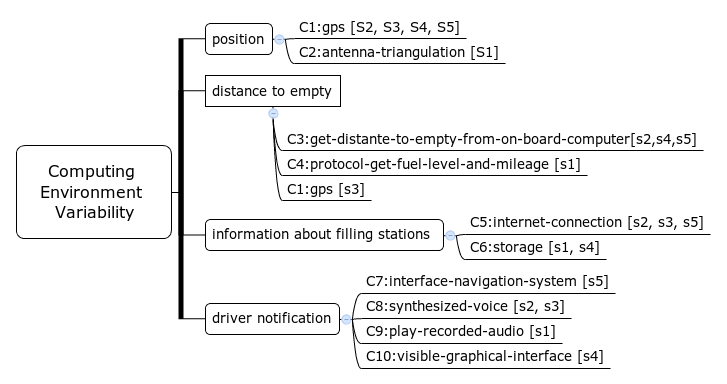
\includegraphics[width=\linewidth]{case_study/comp_env_scearios}
 \caption{Computing Environment Evaluation Scenarios}
\label{fig:variability_scenarios}
\end{figure}


\emph{Question 1.2:  How reliable would a plan provided
by the algorithm be?}: Test cases were created for each scenario (s1-s7).
To validate the algorithm’s correctness,
we verified the generated plans in each test case, asserting if the expected artifacts are in the resulting plan.
For scenarios s1-s5, the planning resulted in valid plans, with the correct artifacts. For scenarios s6 and s7, the algorithm returned NULL, as there is no possible deployment plan for these scenarios. All the tests passed.

\emph{Question 1.3: How long would the algorithm take to come up with a deployment plan?}: In each scenario, the time spent by the algorithm was measured. Table~\ref{table:planning_time} shows the scenarios, the context and time spent for planning in each scenario. In the worst case, it took 9ms to come up with the plan.

\begin{table}[!htb]
\centering
\caption{Time to come up with a plan}
\begin{tabular}{|p{0.7cm}|p{3.75cm}|p{1cm}|}
\hline
  Ref. &
  Context &
  Time \\ \hline

s1 &
C2, C4, C6, C9 &
9ms \\ \hline
s2 &
C1, C3, C5, C8 &
3ms \\ \hline
s3 &
C1, C5, C8 &
1ms \\ \hline
s4 &
C1, C3, C6, C10 &
1ms \\ \hline
s5 &
C1, C3, C5, C7 &
1ms \\ \hline
s6 &
C3, C6, C8 &
1ms \\ \hline
s7 &
C1, C3, C7  &
1ms \\ \hline

\end{tabular}
\label{table:planning_time}
\end{table}

    %
    % \item How does it scale over the amount of artifacts in the component repository?
    % \begin{itemize}
    %   \item time to plan the deployment in.
    %   \item space occupied during the planning.
    % \end{itemize}

\subsection{Scalability Assessment}

To evaluate the algorithm's scalability, we developed other test cases.  A repository with randomly generated artifacts was instantiated. And deployment requests that generate plans with different number of artifacts were made. With this we could evaluate the impact of the generated plan size in the the planning time.
The generated repository had 143,500 artifacts.

A guide to setup the experimental environment and all source code used is available in a repository on github.
\footnote{The needed source code and a step by step guide are available at
\url{https://github.com/lesunb/goalp/tree/master/scalability-evaluation} Accessed on December 4th, 2016}

To analyze the experimental results, R Scripts\cite{the_r_foundation_r_2016} were used to handle data and plot graphs. This scripts and the dataset is available in a repository on github.
\footnote{R Scripts and used dataset are available at:
\url{https://github.com/lesunb/goalp/tree/master/scalability-evaluation} Accessed on December 4th, 2016}

\emph{Q2.1: How does the algorithm scale over the number of artifacts in the deployment plan?} We executed 100 deployment planning requests, with different levels of complexity, where the generated plans were composed of artifacts summing from 40 to 3,100 artifacts.

\begin{figure}[!htb]
  \centering
  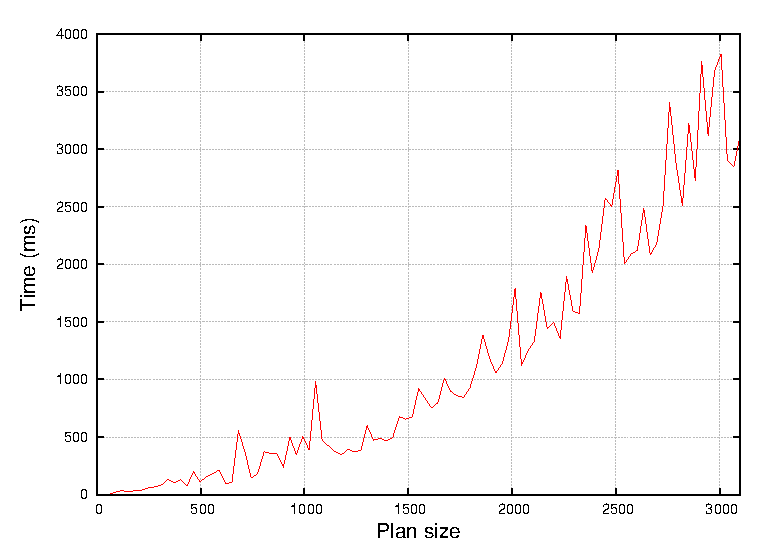
\epsfig{file=results/planning/plan_size_vs_time.eps, width=5.2in}
  \caption{Scalability over the size of plan}
\label{graph_plan_size_and_time}
\end{figure}

The observed time in function on the number of artifacts in the plan is shown if figure~\ref{graph_plan_size_and_time}.

\emph{Q2.2:  How does the algorithm scale over the variability level on the repository?} We repeated the experiment for different levels of variability in the repository.
The level meaning the number of artifacts in the repository that provides the same goals, but with different context conditions. The experiments were executed for a variability level varing from 1 to 10.
The result is depicted in figure~\ref{graph_scalability}. Each curve represents a different level of variability.

\begin{figure}[!htb]
  \centering
  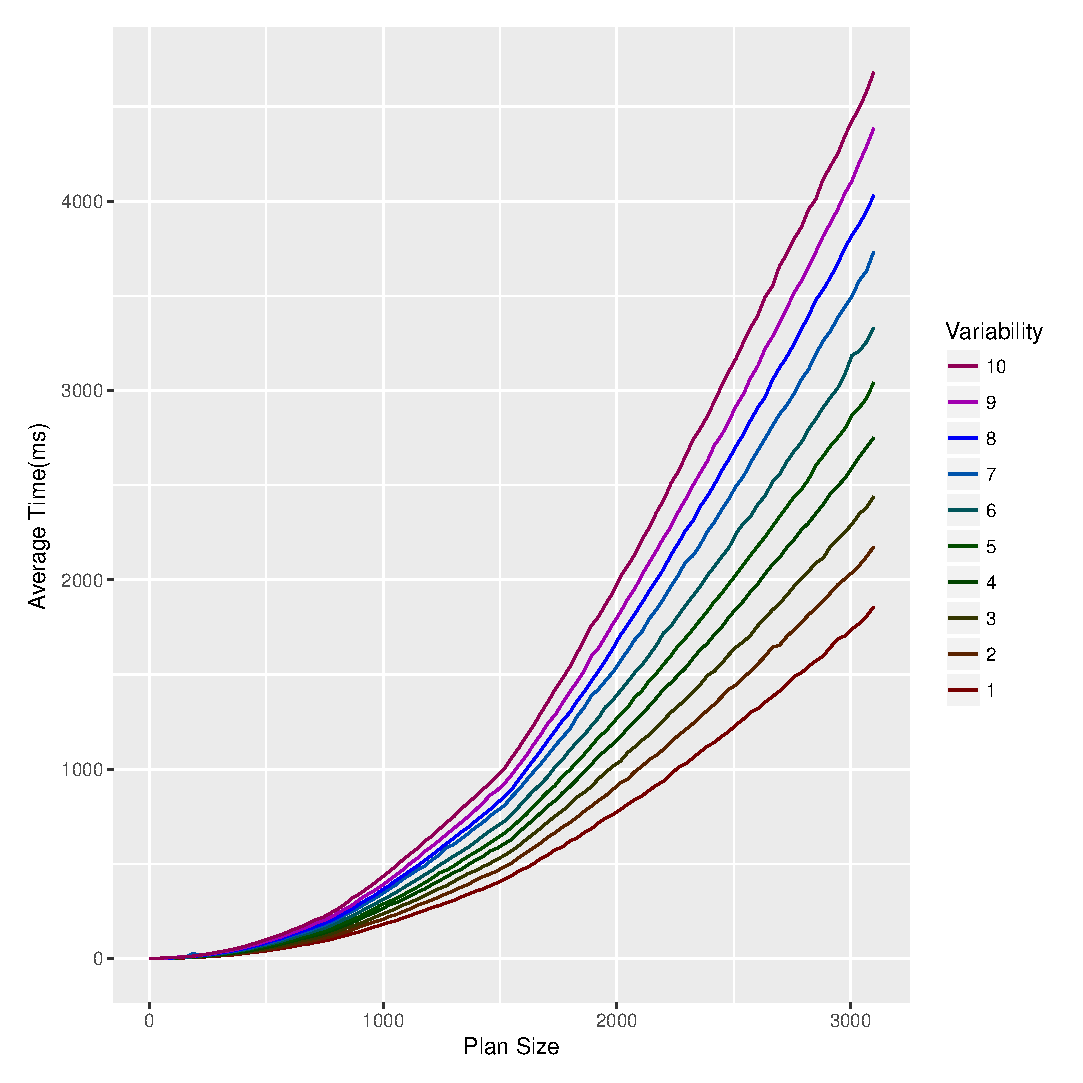
\epsfig{file=results/planning/size_and_variability.eps, width=5.2in}
  \caption{Scalability over variability level - Average (10 executions)}
\label{graph_scalability}
\end{figure}

At the worst case, a deployment that need 3,100 artifacts, with 10 variants for each artifact, took 3.8s to be planned. Requests that required up to 1,000 artifacts could be fulfilled in less then a half-second.

\subsection{Discussion of Results}

In conclusion, the time spent planning the deployment is expect to be negligible in face the time that would take to copy the artifacts from a repository to the target environment.
